\documentclass[12pt]{report}
\usepackage[top=1in, bottom=1in, left=1in, right=1in, a4paper]{geometry}

 \ifx\pdftexversion\undefined
 \usepackage[dvips]{graphicx}
 \else
 
 \usepackage[pdftex]{graphicx}
 \DeclareGraphicsRule{*}{mps}{*}{}
 \fi
%\usepackage{tabularx,colortbl}
\usepackage{url}
\usepackage{chapterbib}
\usepackage{hyperref}
\usepackage{tabularx}
\usepackage{times}
%\usepackage{tikz}
%\usepackage{pgfplots}
%\usepgfplotslibrary{groupplots} 
%\usepackage{pgf, pgfarrows, pgfnodes}
\usepackage{lscape}
\usepackage{longtable}
\usepackage{float}
\usepackage{url}
\usepackage{multicol}
\usepackage{color}
\usepackage{float}
\usepackage{paralist}
%\usepackage[none]{hyphenat}
\renewcommand{\bibname}{References}
\usepackage{listings}
\setcounter{secnumdepth}{4}
\setcounter{tocdepth}{4}
\definecolor{codegreen}{rgb}{0,0.6,0}
\definecolor{codegray}{rgb}{0.5,0.5,0.5}
\definecolor{codepurple}{rgb}{0.58,0,0.82}
\definecolor{backcolour}{rgb}{0.95,0.95,0.92}
\lstdefinestyle{mystyle}{
    backgroundcolor=\color{backcolour},   
    commentstyle=\color{codegreen},
    keywordstyle=\color{magenta},
    numberstyle=\tiny\color{codegray},
    stringstyle=\color{codepurple},
    basicstyle=\footnotesize,
    breakatwhitespace=false,         
    breaklines=true,                 
    captionpos=b,                    
    keepspaces=true,                 
    numbers=left,                    
    numbersep=5pt,                  
    showspaces=false,                
    showstringspaces=false,
    showtabs=false,                  
    tabsize=2
}
 
\lstset{style=mystyle}



\begin{document}

\begin{titlepage}
 \begin{center}
\LARGE
\textbf{Cloud based IT Infra with Central Identity} \\
%\vfill
%\large
%\textbf{\{ Project reboot \}}\\
\vfill
\textbf{Phase II -- Project Report }\\
\vfill
\Large
\underline{\textbf{Project Guide }} \\ 
\large
\underline{} \\
T. Chandra Shekhar \\
\small
Dept. of CSE -- RGUKT Nuzvid \\
\small
chandra.indra@gmail.com
\vfill

\Large
\textbf{\underline{ Project Team } } \\
\underline{} \\
\large
\begin{tabular}{l  l}
T. Aneesh Kumar & N090247  \\
P. Nageswarao  & N091030  \\
P. Anesh  & N090977  \\
P. Jyothi Ram & N090990  \\
K. Naresh Chowdary  & N090331  \\
N. Venkata Sateesh  & N090935  \\
M. Sanyasi Rao & N090891 
\end{tabular}

\vfill



\includegraphics[width=3.5cm]{rgukt_logo.jpg} 
\Large
\underline{} \\
\underline{} \\
\normalsize
\textbf{Dept. of Computer Science and Engg. } \\
\textbf{R.G.U.K.T. - Nuzvid } \\
\textbf{Krishna Dt. - Andrha Pradesh - 521202}


\normalsize
\vfill
%\begin{multicols}{2}
%\begin{flushleft}
%\textbf{Start Date} : Sep 2014 \\
%\end{flushleft}
%
%
%\begin{flushright}
%\textbf{End Date} : Jan 2015 \\
%\end{flushright}
%\end{multicols}

\textbf{Jan 2015 -- Apr 2015 }

\end{center}
\end{titlepage}

% \pagebreak \thispagestyle{empty} \textcolor{white}{text} \pagebreak
 
\chapter*{Abstract}
\setcounter{page}{1}
\pagenumbering{roman}
\normalsize
\hspace{0.5cm} The main objective of ``Cloud based IT Infra with Central Identity'' Phase II is to provide the implementation to our objectives. \newline

We would like to combine Network single sign-on with Web based single sign on along with XtreemFS and HAProxy for fault tolerant load balancing environment\newline

%\pagebreak \thispagestyle{empty} \textcolor{white}{text} \pagebreak

\setcounter{page}{2}
\pagenumbering{roman}
\tableofcontents
\listoffigures
%\listoftables
\pagebreak \thispagestyle{empty} \pagebreak

 
\setcounter{page}{1}
\pagenumbering{arabic}


\chapter{Introduction}

\section{Introduction}
	``Cloud Based IT Infra with Central Identity'' is a complete solution, based on private cloud to enhance and effiecient utilization the IT Infrastructure of an emerging Universities and Organizations with Central Identity for all its users to access its services.\newline

	It is going to be developed in 3 phases 
	\begin{itemize}
		\item \textit{Private cloud} 
		\item \textit{Deploying Network Services} 
		\item \textit{Central Identity}
	\end{itemize}
	
\subsection{Private Cloud}

	Private Cloud establishment is targeted for hardware resource pooling, providing high computational and scalable virtual machines for deploying network based applications (smtp, proxy, ftp), web application and Network storage.
	
\subsection{Deploying Network Services}

	Configuration of Uniform hardware experience over the complete university includes single sign on on every device, configuration of mail servers etc.
	
\subsection{Central Identity}

	Essential part that combines normal network services(proxy, mail, etc.) and organizational web \& native applications. In addtion to that this central identity is available to thrid party developers as API with dynamic based role user authentication protocols.	
	
\chapter{Phase I Work}

	As part of Phase I, we have done literature survey and anlyzed feasability of the several components
	
\section{Components}

	\begin{itemize}
		\item Central Identity
		\begin{itemize}
			\item Single Sign-On with REST API
			\item Identity Management
			\item Dynamic Role Based Access Control
		\end{itemize}
		\item Network Based Central Identity
		\begin{itemize}
			\item LDAP Servers
			\item NFS Servers
		\end{itemize}
		\item Cloud Computing
		\begin{itemize}
			\item 	Cloud Characterstics
			\item Service Models 
			\item Deployment Models 
		\end{itemize}		 
		\item Private Clouds 
		\begin{itemize}
		 	\item Introduction 
			\item Open Source Tools 
		\end{itemize}			

	\end{itemize}

\chapter{Phase II Work}

	As part of Phase II, we have tried to implement some of the above mention components 

\section{Components}

	\begin{itemize}
		\item Web based Signle Sign On
		\begin{itemize}
			\item OAuth Provider 
			\item University Users Profiles 
			\item REST API 
			\item Support of assigin roles to users with their permission set
			\item Testing oauth client library in PHP using php-curl
		\end{itemize}
		\item Network Components
		\begin{itemize}
			\item LDAP Server
			\item NFS Server
			\item Haproxy
			\item GlusterFS
			\item XtreemFS
			%\item DOS Attacks
		\end{itemize}
		\item Private Infrastructure Cloud
		\begin{itemize}
			\item Openstack Architecture
			\item Installation
			\item Virtual Machines
		\end{itemize}		 			

	\end{itemize}

\chapter{Web based Single Sign-On}

\section{OAuth Provider}
\hspace{6mm} \linebreak Here in this section the overall workflow of Authentication in a Single Sign-On System is explained. In order to Authenticate users with the given credentials we must use a robust and stable protocol. And many Single Sign-On systems uses OAuth protocols for this purpose. Single Sign-On uses OAuth protocol for both Authentication \& Authorization.$ ^{3}$
\subsection{OAuth Protocol}
OAuth is an authentication protocol that allows users to approve application to act on their behalf without sharing their password.
The below figure explains the flow of Authentication in OAuth Protocol. $ ^{5}$
\begin{figure}[H]
\begin{center}
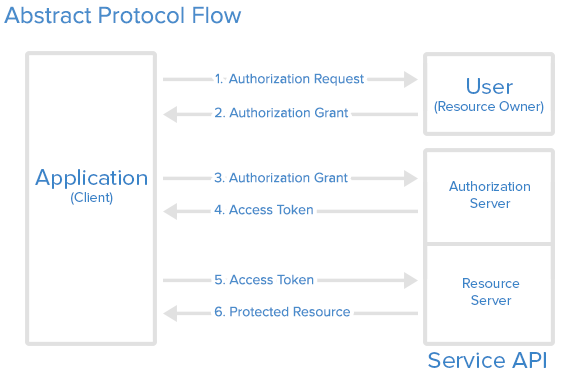
\includegraphics[scale=0.5]{abstract_flow}
\caption{OAuth Protocol Work Flow Diagram\label{fig:OAuth Protocol Work Flow Diagram}}
\end{center}
\end{figure}
Steps invloved in the above flow diagram
\begin{itemize}
\item The application requests authorization to access service resources from the user
\item If the user authorized the request, the application receives an authorization grant
\item The application requests an access token from the authorization server (API) by presenting authentication of its own identity, and the authorization grant
\item If the application identity is authenticated and the authorization grant is valid, the authorization server (API) issues an access token to the application. Authorization is complete.
\item The application requests the resource from the resource server (API) and presents the access token for authentication
\item If the access token is valid, the resource server (API) serves the resource to the application
\end{itemize}
%\subsection{How well we implemented this?}
%\hspace{6mm} 
%To implement OAuth provider we used python-django with oauth-tool-kit. When user requests the protected resource, oauth-tool-kit will generate client id and client secret. By using those user will get access token to access protected resource. 
\section{University User Profiles}
\begin{figure}[H]
\begin{center}
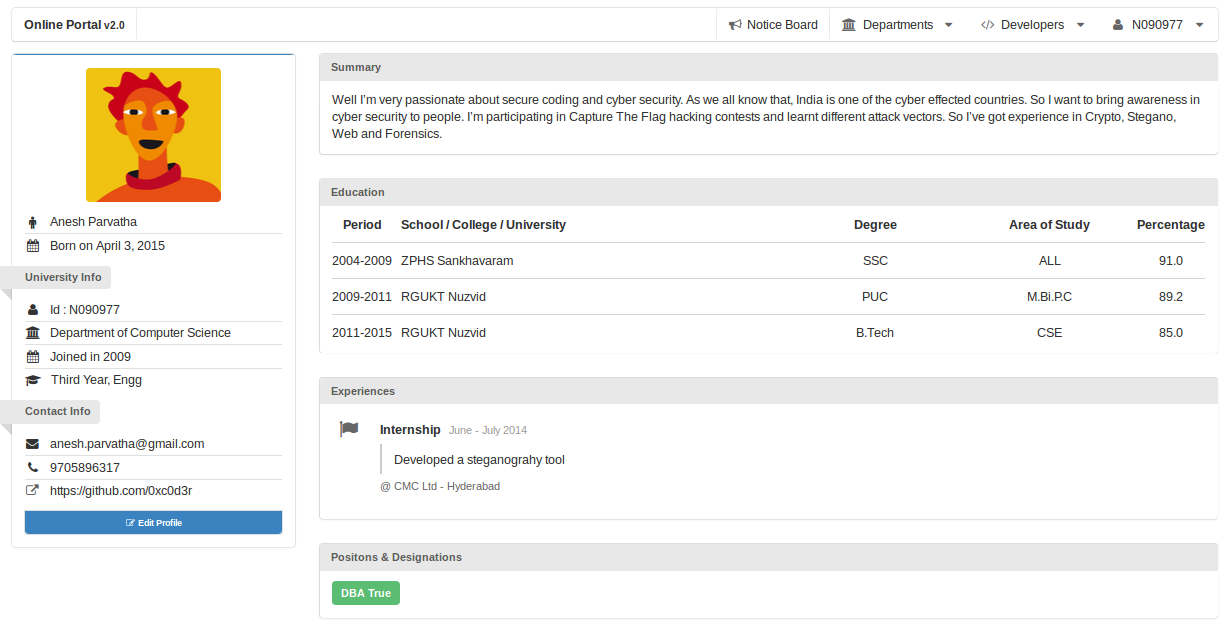
\includegraphics[scale=0.4]{RID_Pics/Profile}
\caption{User Profile\label{fig:User Profile Section}}
\end{center}
\end{figure}
\begin{figure}[H]
\begin{center}
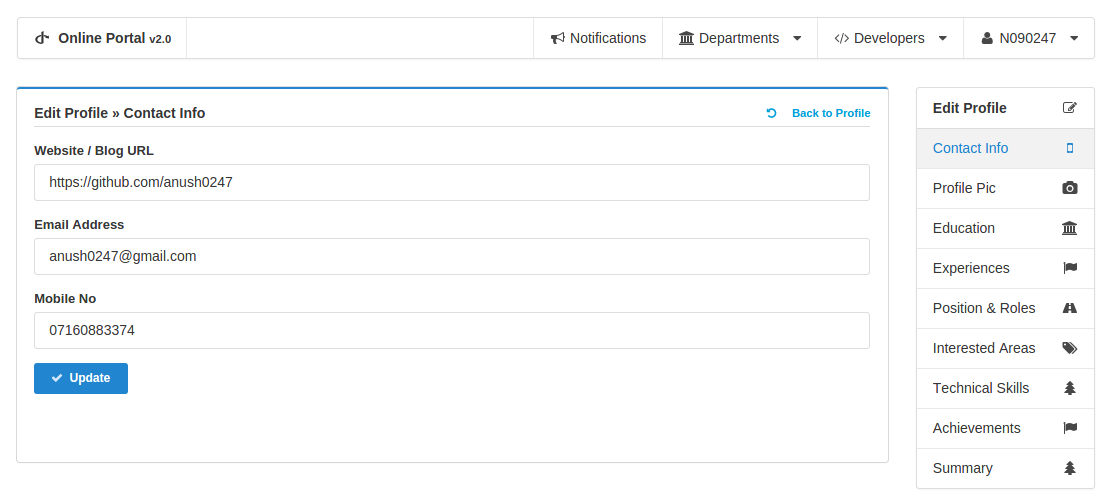
\includegraphics[scale=0.4]{RID_Pics/Edit_Profile}
\caption{Edit User Profile\label{fig:Edit User Profile}}
\end{center}
\end{figure}
\section{REST API} 
\hspace{6mm}REST stand for \textbf{RE}presentational \textbf{S}tate \textbf{T}ransfer. It's a collection of simple URIs, and HTTP calls like GET,PUT,POST,DELETE to those URIs to get some Protected data from a Resource Server. Once User provides a set of valid credentials to OAuth Provider it will generate an access token to that particular user, with that token user can fetch protected resources from the resource server by making basic HTTP calls through REST API. REST API provides users a flexibility to perform Basic CRUD(Create,Read,Update,Delete) on resource server.$ ^{4}$
	\begin{figure}[H]
	\begin{center}
	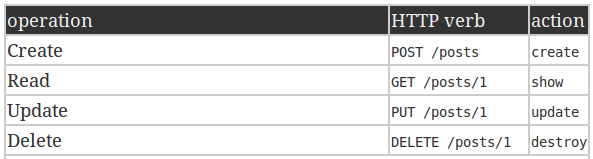
\includegraphics[width=7cm,height=2cm]{CRUD}
	\caption{CRUD Operations\label{fig:CRUD Operations}}
	\end{center}
	\end{figure}
\subsection{Technologies Used}
\begin{itemize}
	\item django $ >= $ 1.6.0
	\item SQLite3
	\item django-rest-framework
	\item oauth-tool-kit
	\item semantic ui 2.0
\end{itemize}
\pagebreak
\subsection{API Testing}
\textbf{\url{/api/basic_info/?access_token=<token>}}
\lstinputlisting[language=Java]{basic_info.json} 
\underline{} \newline
\textbf{\url{/api/contact_info/?access_token=<token>}}
\lstinputlisting[language=Java]{contact_info.json}
\underline{} \newline
\textbf{\url{/api/education/?access_token=<token>}}
\lstinputlisting[language=Java]{education.json}
\underline{} \newline
\textbf{\url{/api/skills/?access_token=<token>}}
\lstinputlisting[language=Java]{skills.json}
\underline{} \newline
\textbf{\url{/api/roles/?access_token=<token>}}
\lstinputlisting[language=Java]{roles.json}
\underline{} \newline


\section{Roles \& Permissions}
\begin{figure}[H]
\begin{center}
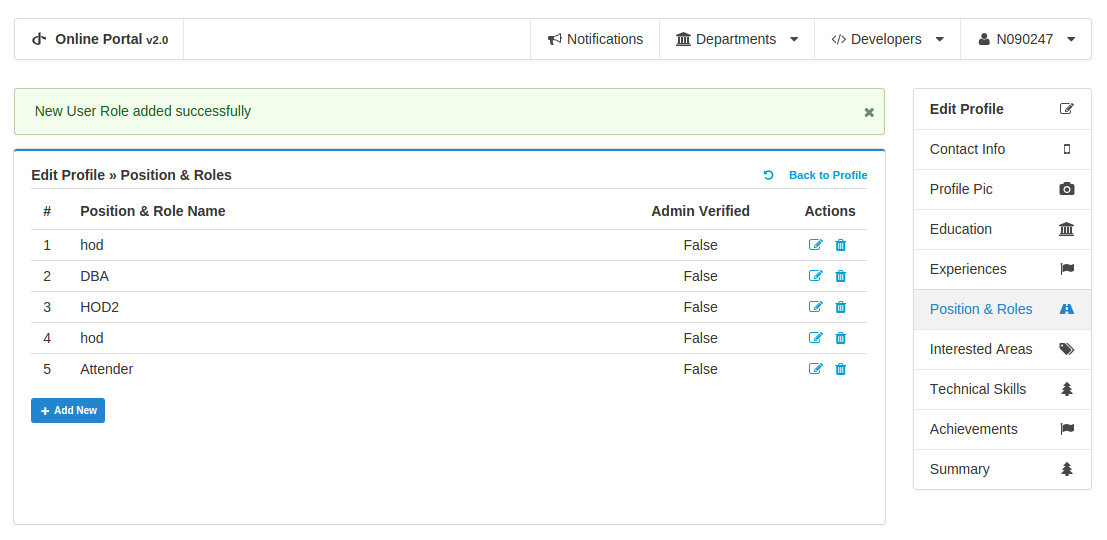
\includegraphics[scale=0.4]{RID_Pics/Roles}
\caption{List of Roles of User\label{fig:User Roles}}
\end{center}

\begin{center}
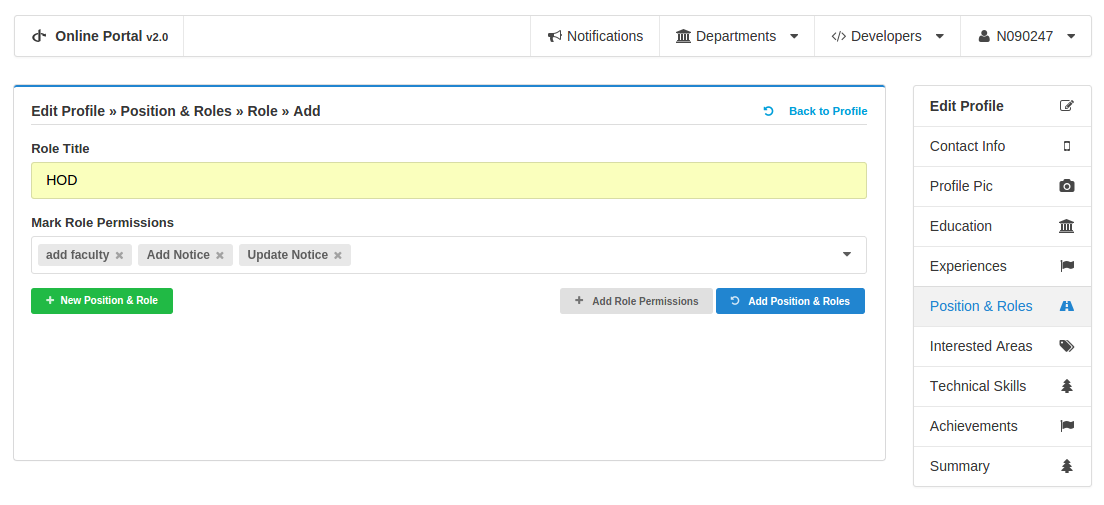
\includegraphics[scale=0.4]{RID_Pics/Add_Permission}
\caption{Adding Permissions Option\label{fig:Add Permissions}}
\end{center}
\end{figure}
\pagebreak
\section{PHP Client Libraray}
\hspace{6mm}  We developed a Client Library for PHP Applications. We used PHP-cURL to perform all the http calls and post requests to get protected data from API Server. And We developed it in a modular way with Object-Oriented approach. And all the function calls in the PHP library is self-explanatory.
\subsection{Initializing the Client Library}
\lstinputlisting[language=php]{init.php}
\subsection{Get Authorization URL}
\lstinputlisting[language=php]{getURL.php}
\subsection{Get Access Token}
\lstinputlisting[language=php]{getToken.php}
\subsection{Initializing API with Access Token}
\lstinputlisting[language=php]{initAPI.php}
\subsection{Getting User Info from API}
\lstinputlisting[language=php]{getInfo.php}

	
	
\chapter{Network Single Sign-On}
\section{Introduction}
	
	Single sign-on (SSO) is a session/user authentication process that permits a user to enter one name and password in order to access multiple applications. The process authenticates the user for all the applications they have been given rights to and eliminates further prompts when they switch applications during a particular session.\\
	\underline{} \newline
	\textbf{Components Used:} 
	\begin{itemize}
	\item LDAP Server
	\item phpLdapAdmin
	\item LDAP Client
	\item HAProxy
	\item GlusterFS
	\item XtreemFS
	\end{itemize}
	
\pagebreak

\section{LDAP Server}

	LDAP, or Lightweight Directory Access Protocol, is a protocol for managing related information from a centralized location through the use of a file and directory hierarchy. It functions in a similar way to a relational database in certain ways, and can be used to organize and store any kind of information. LDAP is commonly used for centralized authentication.

\subsection{Installation and Configuration $ ^{9}$}
	The OpenLDAP server is in Ubuntu's default repositories under the package "slapd". We have to install some additional utilities in order to use it in full pledged way. 
	
	\begin{itemize}
	\item sudo apt-get \textbf{update}
	\item sudo apt-get install \textbf{slapd ldap-utils}
	\end{itemize}

	After the installation is complete, we actually need to reconfigure the LDAP package by the following
	\begin{itemize}
	\item sudo \textbf{dpkg-reconfigure slapd}
	\end{itemize}

		By following below steps we have to configure the LDAP
	\begin{itemize}
		\item Omit OpenLDAP server configuration? \textbf{No}
		\item DNS domain name? \textbf{reboot.org}
		\item Organization name? \textbf{reboot}
		\item Administrator password? \textbf{Password}
		\item Database backend to use? \textbf{HDB}
		\item Remove the database when slapd is purged? \textbf{No}
		\item Move old database? \textbf{Yes}
		\item Allow LDAPv2 protocol? \textbf{No}
	\end{itemize}
	
\pagebreak
	
\section{phpLDAPadmin}	
	
	It’s a web-based LDAP client. It provides easy, anywhere-accessible, multi-language administration for LDAP server. By this configuration and monitor of LDAP Server will be done in an easy way. \\
\underline{} \newline
Its hierarchical tree-viewer and advanced search functionality make it intuitive to browse and administer your LDAP directory. Since it is a web application, this LDAP browser works on many platforms, making your LDAP server easily manageable from any location.
\subsection{Installation and Configuration}
	\begin{itemize}
	\item sudo apt-get install \textbf{phpldapadmin}
	\end{itemize}
	
	After the installation is complete configuration will be done by making following changes in the
config.php file of phpLDAPadmin.
	\begin{itemize}
	\item sudo nano \textbf{/etc/phpldapadmin/config.php}
	\end{itemize}

	\lstinputlisting[language=PHP,caption=PHP Config file]{conf.php}

\subsection{Web Interface of phpLDAPadmin:}
	%\subsubsection{Authentication:}
\begin{multicols}{2}
\begin{flushleft}

		\begin{figure}[H]
		\begin{center}
		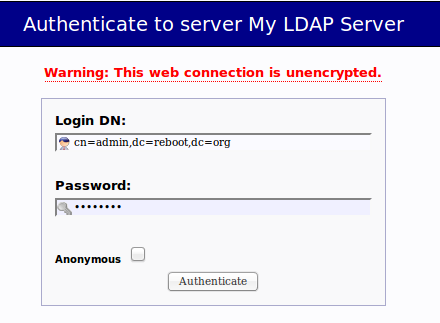
\includegraphics[width=6cm,height=6cm]{Screens/LdapServerLogin.png}
		\caption{phpLDAP \label{fig: phpLDAP }}
		\end{center}
		\end{figure}

\end{flushleft}
\begin{flushright}

		\begin{figure}[H]
		\begin{center}
		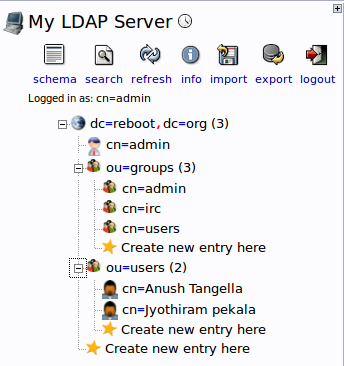
\includegraphics[width=6cm,height=6cm]{Screens/serversidebar.png}
		\caption{Complete category of LdapServer \label{fig: Complete category of LdapServer}}
		\end{center}
		\end{figure}
	

\end{flushright}
\end{multicols}


	%\subsubsection{Server’s sidebar with complete information:}
		
	%\subsubsection{User Creation in LDAP server:}
		\begin{figure}[H]
		\begin{center}
		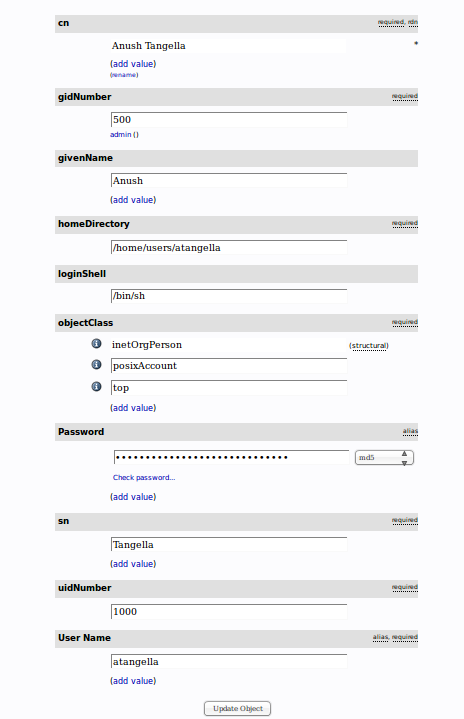
\includegraphics[width=10cm,height=15cm]{Screens/UserCreation.png}
		\caption{User Creation \label{fig: User Creation}}
		\end{center}
		\end{figure}

	%\subsubsection{Creating Group:}	
		\begin{figure}[H]
		\begin{center}
		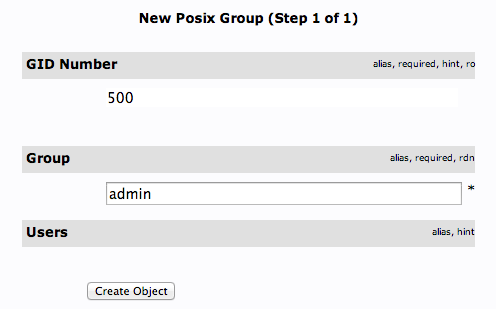
\includegraphics[width=8cm,height=6cm]{Screens/admin_group.png}
		\caption{Group Creation \label{fig: Group Creation}}
		\end{center}
		\end{figure}		
		
	%\subsubsection{Adding user to Group:}
		\begin{figure}[H]
		\begin{center}
		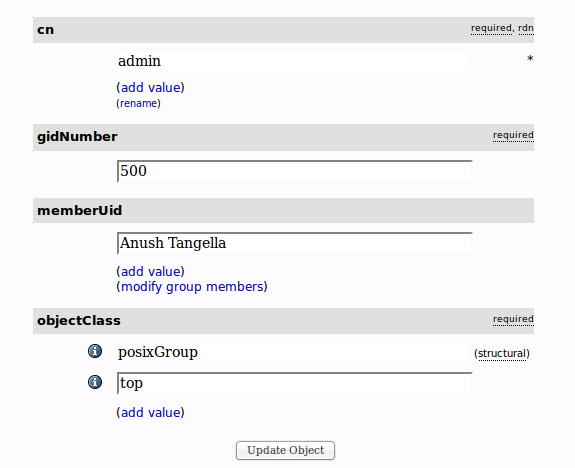
\includegraphics[width=10cm,height=8cm]{Screens/AddUsertoGroup.png}
		\caption{Adding User to Group \label{fig: Adding User to Group}}
		\end{center}
		\end{figure}
		
	%\subsubsection{Groups complete information:}
		\begin{figure}[H]
		\begin{center}
		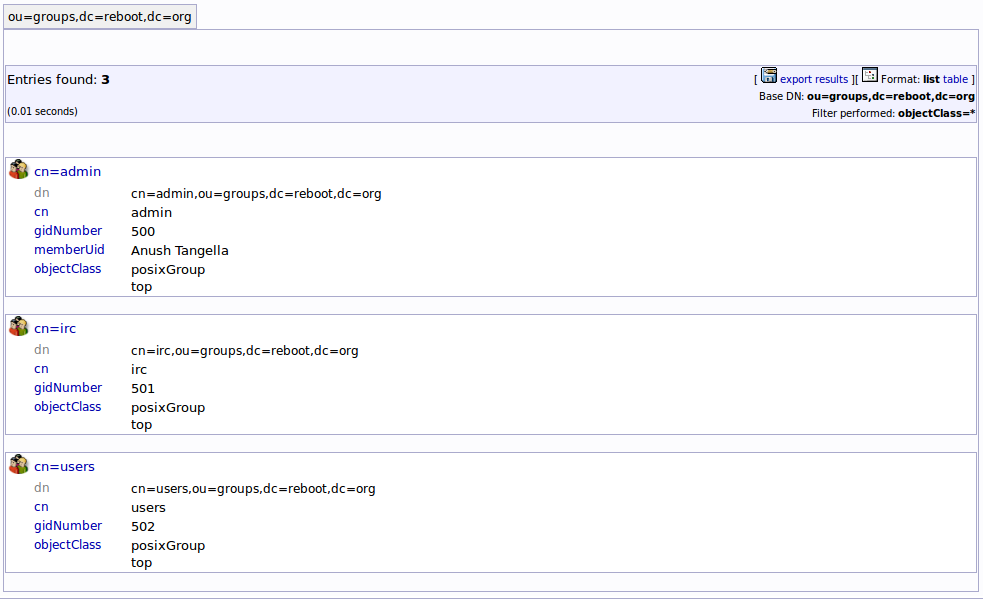
\includegraphics[width=17cm,height=10cm]{Screens/Groupsinfo.png}
		\caption{Groups information \label{fig:Groups information}}
		\end{center}
		\end{figure}
		
\section{LDAP Client:}		
	LDAP, or Lightweight Directory Access Protocol, is one way of keeping authentication information in a single centralized location. We need another droplet to act as the client machine.
	\subsection{Installation and Configuration:}
		On the client machine, we need to install a few packages to make authentication function correctly with an LDAP server.	
		\begin{itemize}
		\item sudo apt-get install \textbf{libpam-ldap nscd}
		\end{itemize}		 
By following these below steps we need to configure the LDAP Client
		\begin{itemize}
		\item LDAP server Uniform Resource Identifier: \textbf{ldap://10.4.34.47/} from \textbf{``ldapi:///''}		
		\end{itemize}

		Distinguished name of the search base:
		This should match our values in LDAP server's /etc/phpldapadmin/config.php file.
		\begin{itemize}
		\item We have to replace " 'server','base',array " within the file to \textbf{``dc=reboot,dc=org''}
		\item LDAP version to use:\textbf{ 3}
		\item Make local root Database admin: \textbf{Yes}
		\item Does the LDAP database require login? \textbf{No}
	 	\item LDAP account for root:
		 	\begin{itemize}
	 		\item This should also match with our values in your \textbf{/etc/phpldapadmin/config.php}
			\item Search for: \textbf{`` ` login ' , ` bind\_id ' '' } within the file
			\item Our example was \textbf{``cn=admin,dc=reboot,dc=org''}
		 	\end{itemize}
		\end{itemize}
		LDAP root account password: \textbf{Our-LDAP-root-password}
		\\
		\linebreak
		If made a mistake and need to change a value, we can go through the menu again by issuing this command:
		\begin{itemize}
		\item sudo \textbf{dpkg-reconfigure ldap-auth-config}
		\end{itemize}
		
		To configure client we adjust a few files that they can look to our LDAP server for authentication information.
		First, we have to edit the /etc/nsswitch.conf file. This will allow us to specify that the LDAP credentials should be modified when users issue authentication change commands
		\begin{itemize}
		\item sudo nano \textbf{/etc/nsswitch.conf}
		\end{itemize}
		\pagebreak
		The three lines we are interested in are the "passwd", "group", and "shadow" definitions. 
		Modify them to look like this:
		\lstinputlisting[language=sh,caption=Config file]{nsswitch.conf}
		
		We have to add the values to our PAM configuration.
		
		PAM, or Pluggable Authentication Modules, is a system that connects applications that can provide authentication to applications that require authentication.
		When we installed and configured our LDAP PAM module, most of the needed information was added to the configuration files and we need to edit below file.
		\begin{itemize}
		\item sudo nano \textbf{/etc/pam.d/common-session}
		\item sudo nano \textbf{/etc/pam.d/login}
		\item sudo nano \textbf{/etc/pam.d/lightdm}
		\end{itemize}
		
	We have to add the below piece of code to each of the above PAM configuration files
		\begin{itemize}
		\item session required \textbf{pam\_mkhomedir.so skel=/etc/skel umask=0022x}
		\end{itemize}
		
		The above will create a home directory on the client machine when an LDAP user logs in who does not have a home directory.
		We have to restart a service for these changes to be implemented:
		\begin{itemize}
		\item sudo \textbf{/etc/init.d/nscd restart}		
		\end{itemize}
		
		\subsection{Log In as an LDAP User:}
		We have now configured our client machine enough to be able to log in as one of our LDAP users. This user does not have to exist on the client machine.
		In order to connect to LDAP Client, we have to ssh into that particular machine.
		\begin{itemize}
		\item ssh \textbf{atangella@10.4.34.45}
		\end{itemize}
\pagebreak
\section{HAProxy}
HAProxy(High Availability Proxy) is an open source load balancer which can load balance any TCP service. It is particularly suited for HTTP load balancing as it supports session persistence and layer 7 processing. HAProxy can be configured as a front-end to load balance two VPS through private network connectivity.\\
\subsection{Installing HAProxy $ ^{8}$}
\# to install haproxy\\
sudo apt-get install haproxy\\
\# to get started by init script\\
edit /etc/default/haproxy, set ENABLED option to 1\\
\# using haproxy\\
sudo /etc/init.d/haproxy {start|stop|reload|restart|status}\\
\subsection{Configuring HAProxy}
edit gedit /etc/haproxy/haproxy.cfg\\
\\
frontend sunny\\
   bind 10.4.34.250:8080\\
   default\_backend sunny-backend\\
backend sunny-backend\\
   balance roundrobin\\
   mode tcp\\
   server sunny 10.4.34.250:80 check\\
   server ram 10.4.34.242:80 check\\
   server knc 10.4.34.245:80 check\\
\\
Requests come to frontend PC will be send to any one of the backend PC's based on the algorithm. Here algorithm can be roundrobin, leastconn.\\

\pagebreak
\section{GlusterFS}
	GlusterFS is a unified, poly-protocol, scale-out file system serving many peta bytes of data. While many databases and other software allows you to spread data out in the context of a single application, other systems can operate on the file system level to ensure that data is copied to another location whenever it is written to disk. A clustered storage solution like GlusterFS provides this exact functionality.\\
\\
	We are writing by considering three systems. we are considering the two of our machines as cluster members and the third as a client. We will be configuring the computers we labeled as gluster0 and gluster1 as the cluster components. We will use gluster2 as the client. $ ^{8}$
\subsection{Configure DNS solution}
Go to \textbf{sudo nano /etc/hosts} and add below lines\\
\#first\_ip gluster0.droplet.com gluster0\\
\#second\_ip gluster1.droplet.com gluster1\\
\#third\_ip gluster2.droplet.com gluster2\\

\subsection{Install server components}
\# On our cluster member machines (gluster0 and gluster1), we can install the GlusterFS server package\\
sudo apt-get install glusterfs-server\\
\#On one of the hosts, we need to peer with the second host. \\ 
sudo gluster peer probe gluster1.droplet.com\\
\subsection{Create a storage volume}
\#Creating and enabling replication property for volume1\\
sudo gluster volume create volume1 replica 2 transport tcp gluster0.droplet.com:/gluster-storage gluster1.droplet.com:/gluster-storage force\\
\#And we can activate the storage by command\\
sudo gluster volume start volume1\\
\subsection{Install and configure client components}
\#On our client machine, we can install the GlusterFS client package\\
sudo apt-get install glusterfs-client\\
\#for mounting our remote storage volume on our client computer\\
sudo mkdir /storage-pool\\
sudo mount -t glusterfs gluster0.droplet.com:/volume1 /storage-pool\\
\subsection{Restrict access to the volume}
\#for restriction of storage volume for clients\\
sudo gluster volume set volume1 auth.allow *\\
\#for removing restrictions\\
sudo gluster volume set volume1 auth.allow gluster\_client1\_ip,gluster\_client2\_ip\\
\\
At this point, you should have a redundant storage system that will allow us to write to two separate servers simultaneously. This can be useful for a great number of applications and can ensure that our data is available even when one server goes down. But GlusterFS is failing in distributed environment at some situations. For that we moved an efficient one XtreemFS, which works very well in distributed environment and tackles all errors.\\
\pagebreak
\section{XtreemFS}
XtreemFS is a fault-tolerant distributed file system for all storage needs. It is simple to setup as it does not use any kernel modules. It's easy to integrate with clients for Linux and Windows. XtreemFS is also a parallel, object-based file system. You can stripe your files across many storage servers for high-performance parallel access. The stripe width can be configured per file.\\
\\
It can stripe files within your cluster and can replicate your data across clusters. This allows you to have high-performance access within your cluster and to share your data in your virtual organization.\\
\\
XtreemFS' replication is fault-tolerant. A broken hard drive or unhealthy storage server does not result in data loss or even degraded service quality. \\
\\
This matters if you have 10 or 1000s of machines, as your jobs finish without interruptions and you can delay repairs to whenever you have time.\\
\subsection{Installation, Creating \& Mounting Filesystem}
\begin{itemize}
\item Added the XtreemFS repo to our system and then installed the packages xtreemfs-server and xtreemfs-client.
\item Starting the Directory Service: \$sudo /etc/init.d/xtreemfs-dir start 
\item Starting the Metadata Server: \$sudo /etc/init.d/xtreemfs-mrc start
\item Starting OSD: \$sudo /etc/init.d/xtreemfs-osd start
\item Loading the FUSE kernel module: \$sudo modprobe fuse
\item We can check the registry by opening the DIR status page in our web browser at http://localhost:30638
\item Creating a new volume with default settings : \$sudo mkfs.xtreemfs localhots/myVolume
\item Creating mounting point : \$sudo mkdir ~/xtreemfs
\item Mounting XtreemFS: \$sudo mount.xtreemfs localhost/myVolume ~/xtreemfs
\item We can unmount using : \$sudo umount.xtreemfs ~/xtreemfs
\end{itemize}
\subsection{Distributed Step}
We assume a setup with two machines:
\begin{itemize}
\item One system running the directory service (DIR), metadata server (MRC), storage server (OSD).
\item Another system running the only storage server (OSD).
\end{itemize}
First, installed the binary packages using repositories made available by the XtreemFS team. Once the repository file is registered, we can install these packages:\\
\\
sudo apt-get install xtreemfs-client xtreemfs-server xtreemfs-tools\\
\\
Now suppose one server to host the DIR and MRC service is called osd1, and my OSDs will be running on osd1 and osd2. On osd2, we have to edit the following config files under /etc/xos/xtreemfs and \textbf{set dir\_service.host = kdc01}. For the mrc and osd config files, we have to set up \textbf{hostname = kdc01}
\begin{itemize}
\item mrcconfig.properties
\item osdconfig.properties
\end{itemize}
On WKS01 where a second OSD will be running, edited the osd config file, point \textbf{dir\_service.host = kdc01} and \textbf{hostname = wks01}
\begin{itemize}
\item osdconfig.properties
\end{itemize}
Then we have to start the services. On KDC01, the following services are started:\\
\\
sudo /etc/init.d/xtreemfs-dir start\\
sudo /etc/init.d/xtreemfs-mrc start\\
sudo /etc/init.d/xtreemfs-osd start\\
\\
On WKS01, OSD service \\
\\
sudo /etc/init.d/xtreemfs-osd start\\
\\
Then we created the XtreemFS filesystem using following commands:\\
\\
sudo mkfs.xtreemfs kdc01/myVol \# on KDC01\\
sudo mount.xtreemfs kdc01/myVol /data \# on KDC01 and WKS01\\
\\
By default, 1 replica will be stored on the entire XtreemFS volume. XtreemFS client is smart enough to contact the best OSD for the file resource. In case it’s desirable to maintain more than 1 replica of the same file, it can be done with the xtfsutil tool. For example, to configure XtreemFS to replicate a file to all available OSDs:\\


\chapter{Private Infrastructure Cloud}
To support this central identity both the network and web network central identity we want to go for the private cloud deployment it includes creating the Private Infrastructure Cloud with openstack and creating Virtual Machines for instaling these services and assign them the IP address.

\section{Openstack Architecture}
Openstack is a cloud operating system that provides the 3 main services for the Infrastructure clouds namely Stoage, Compute, Networking and some other components are can be added later as addons
\underline{} \newline
\begin{figure}[H]
	\begin{center}
	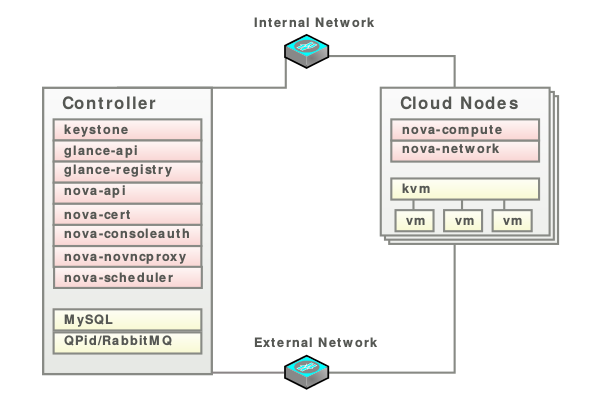
\includegraphics[width=11cm,height=8cm]{./openstack_1.png}
	\caption{ Openstack Architecture.\label{fig:Openstack Architecture }}
	\end{center}
\end{figure}

\section{Installation}

Installing openstack includes component wise installation namely NTP, MySQL, Rabbitmq-Server, Keystone, Nova, Cinder, Glance, Neutron

\begin{figure}[H]
	\begin{center}
	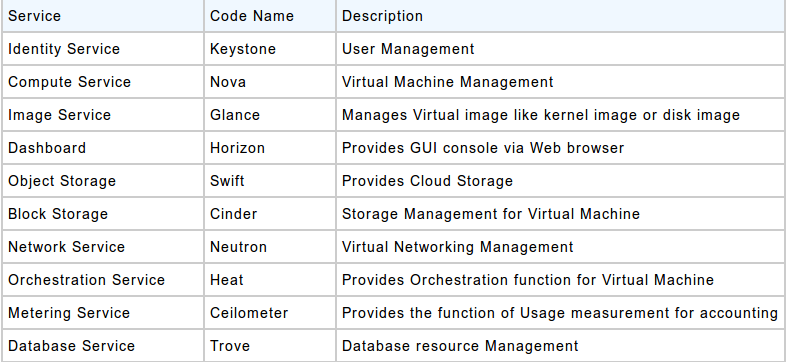
\includegraphics[width=14cm,height=5.5cm]{./openstack_4.png}
	\caption{ Openstack Service Components. $^{12}$ \label{fig:Openstack Service Components }}
	\end{center}
\end{figure}

\subsection{NTP}
\# apt-get install ntp
\subsection{MySQL}
\# apt-get install mysql-server
\subsection{Rabbitmq-server}
\# apt-get install rabbitmq-server
\subsection{Keystone}
\# apt-get install keystone
\subsection{Glance}
\# apt-get install glance python-glanceclient
\subsection{Nova}
\# apt-get install nova-api nova-cert nova-conductor nova-consoleauth nova-novncproxy nova-scheduler python-novaclient
\subsection{Neutron}
\# apt-get install neutron-server neutron-plugin-ml2
\pagebreak
\section{Virtual Machines}
This Virtual Machines are created from the resource pool after successfull installation openstack
\begin{figure}[H]
	\begin{center}
	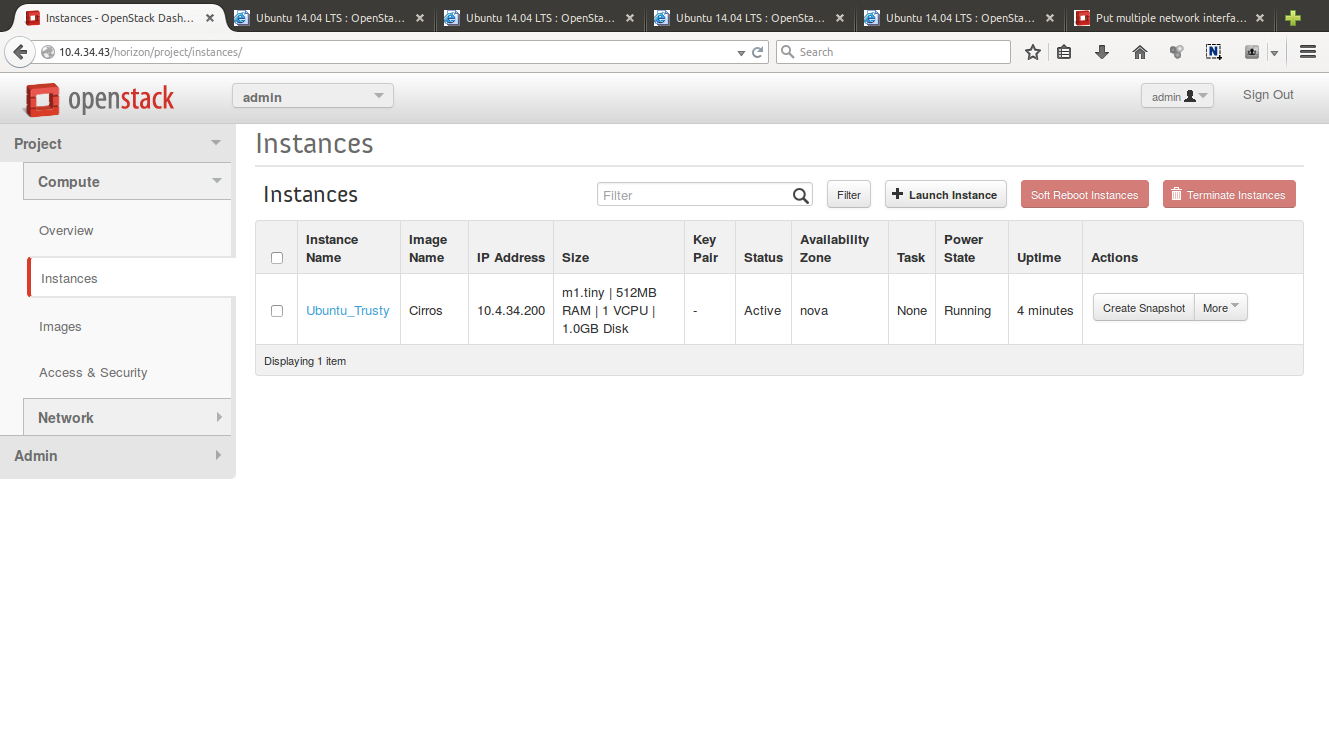
\includegraphics[width=12cm,height=8cm]{./openstack_2.png}
	\caption{ Openstack Virtual Machines.\label{fig:Openstack Virtual Machines }}
	\end{center}
\end{figure}
\begin{figure}[H]
	\begin{center}
	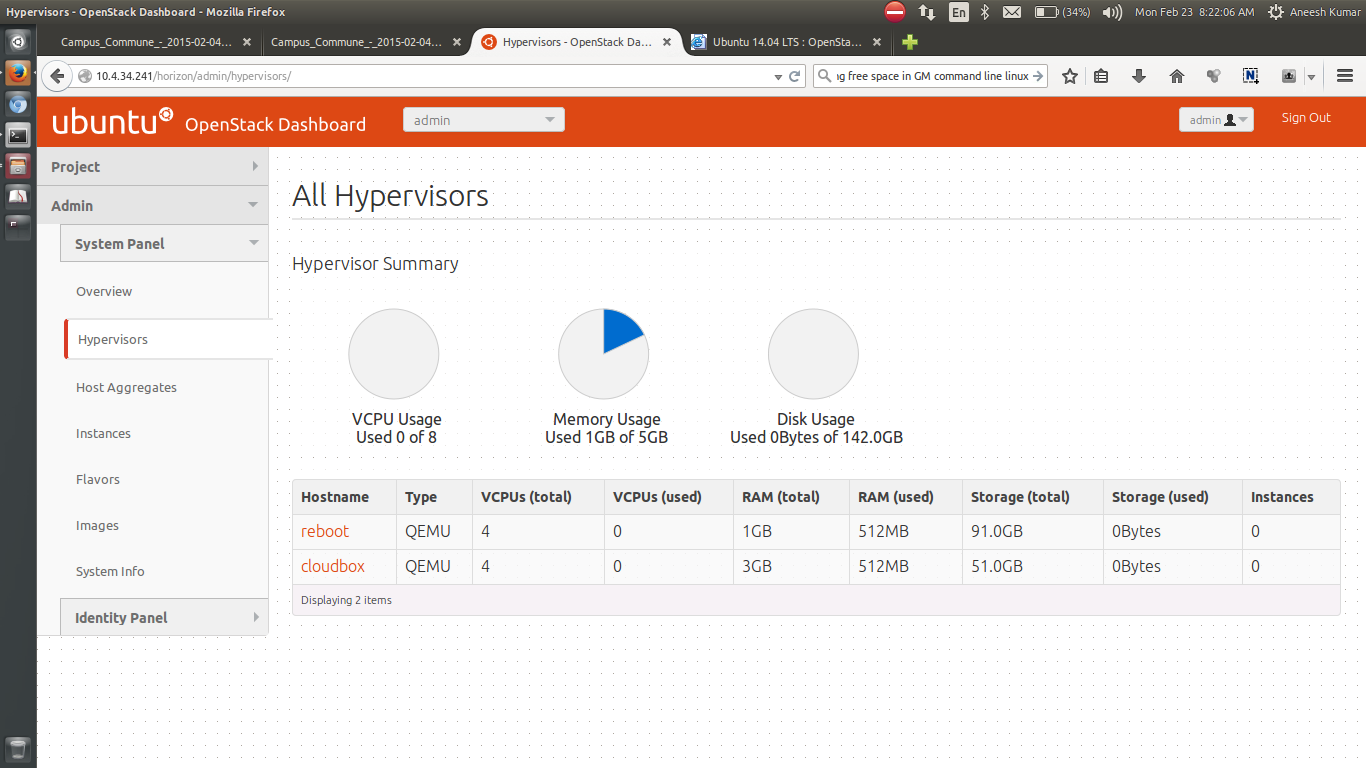
\includegraphics[width=12cm,height=8cm]{./openstack_3.png}
	\caption{ Openstack Resource Pool.\label{fig:Openstack Resource Pool }}
	\end{center}
\end{figure}
\chapter{Conclusion \& Future Work}
\section{Conclusion} 
We tried GlusterFS for replication among systems, but it’s not working if any one of the system fails. Then we found that XtreemFS works well in distributed system and provides fault tolerant solution. \newline
\underline{} \newline
We developed network based sign on using LDAP and web based single sign on along with REST API using Oauth 2.0 and Django. We tried to create private cloud using openstack but lot of errors came because of proxy based internet and low configured PCs.

\section{Future Work}
We would like to combine Network single sign-on with Web based single sign on along with XtreemFS and HAProxy. Creating virtual machines and Private cloud is not possible with the available systems. But if we could provide systems with enough configuration, sure we can create better sophisticated solution

\chapter{References}
\begin{enumerate}
	\item Django Docs -- \url{https://docs.djangoproject.com/en/1.7/}
	\item Django -- \url{https://djangoproject.com/}
	\item Django OAuth Tool Kit -- \url{https://github.com/evonove/django-oauth-toolkit}
	\item Django REST Framework -- \url{http://www.django-rest-framework.org/}
	\item OAuth 2.0 -- \url{http://oauth.net/2/}
	\item Semantic UI -- \url{http://beta.semantic-ui.com/}
	\item GlusterFS -- \url{https://www.digitalocean.com/How To Create a Redundant Storage Pool Using GlusterFS on Ubuntu Servers _ DigitalOcean.htm}
	\item HAProxy -- \url{www.digitalocean.com/How To Use HAProxy to Set Up HTTP Load Balancing on an Ubuntu VPS _ DigitalOcean.htm}
	\item LDAP -- \url{https://www.digitalocean.com/community/tutorials/how-to-install-and-configure-a-basic-ldap-server-on-an-ubuntu-12-04-vps}
	\item NFS Server -- \url{http://www.server-world.info/en/note?os=Ubuntu_14.04&p=nfs}
	\item NFS Client -- \url{http://www.server-world.info/en/note?os=Ubuntu_14.04&p=nfs&f=2}
	\item Openstack -- \url{http://www.server-world.info/en/note?os=Ubuntu_14.04&p=openstack_icehouse}
\end{enumerate}

\end{document}